HSB
how platooning was implemented/3 sec rule

\section{Traffic Sim, pre-project}
For my master's pre-project I worked on a traffic simulator which controls the ChIRP robots.
The traffic simulator is a project for Statens Vegvesenet Teknologidagene in Trondheim where the ChIRP Robots were used to demonstrate the concept of platooning. 
The idea of platooning is to use an autonomous system (either global centralized system or each individual entity communicates with each other) to control the vehicles as one unit thus increasing the flow of traffic. These vehicles can be anything, but in this case we imagine them being cars or trucks found in traffic. When the red traffic light changes to green light, drivers usually drive one by one. The driver only drives forward when there is enough space in front of his or her car, in other words, the drivers are trying to follow the 3 second rule.\footnote{\href{http://www.smartmotorist.com/traffic-and-safety-guideline/maintain-a-safe-following-distance-the-3-second-rule.html}{http://www.smartmotorist.com/traffic-and-safety-guideline/maintain-a-safe-following-distance-the-3-second-rule.html}}
However with platooning and autonomous steering/driving the cars will drive instantly when the red light changes to green, and it will look like all the cars drive as one unit, or like a train if you will.
This leads to less air resistance and the cars will be able to cross an intersection much faster. This is considered dangerous if it had been normal humans driving, because driving with almost no gap in between the vehicles would not leave enough time to react and brake in time. With autonomous self driving vehicles it might be possible to platoon without being a risk because all the cars behave as one unit, and when one car brakes or slow down, all the cars behind it will start to brake/slowing down instantly without any reaction time added.

The system we used to demonstrate platooning for Vegvesenet Teknologidagen used a web camera to track all the robots in a sandbox. The sandbox is an empty box with four walls which the robots were able to move freely inside. Using a projector we drew an 8 shaped track on kraft paper which was later painted with black paint. Styrofoam was used to build a city-like environment around the track.
The combination of paint and kraft paper did not work very well due to bulges and the paint being too slippery for the robots, so they were not able to drive around efficiently. Sometimes they got stuck on the bulges or they were not able to turn like they were supposed to do and crashed into the wall.  We therefore had to cut out the painted part, so the robots could drive on the sandbox floor.

All the robots used for the demonstration were equipped with a bluetooth module and 2 circular post-it notes which was light green and pink.
The camera was able to detect these post-it notes using the OpenCV (Open source Computer Vision) and C++ boost library. The software for tracking the robots were already implemented and we only had to set it up on a xubuntu linux machine.
Using these pink and green post-it notes and a web camera, the computer could track the position and rotation of each robot. A parameter of how many robots had to be set beforehand, along with the parameters hue, saturation and brightness (HSB) for the red (in our case pink) and green color. The calibration for the red and green HSB calibration had to be manually set, but the camera tracking software had a calibration mode where we could test whether the parameters we had set was correct or not. These parameters had to be set so the software knew what colors it was looking for.
\begin{figure}
\centering
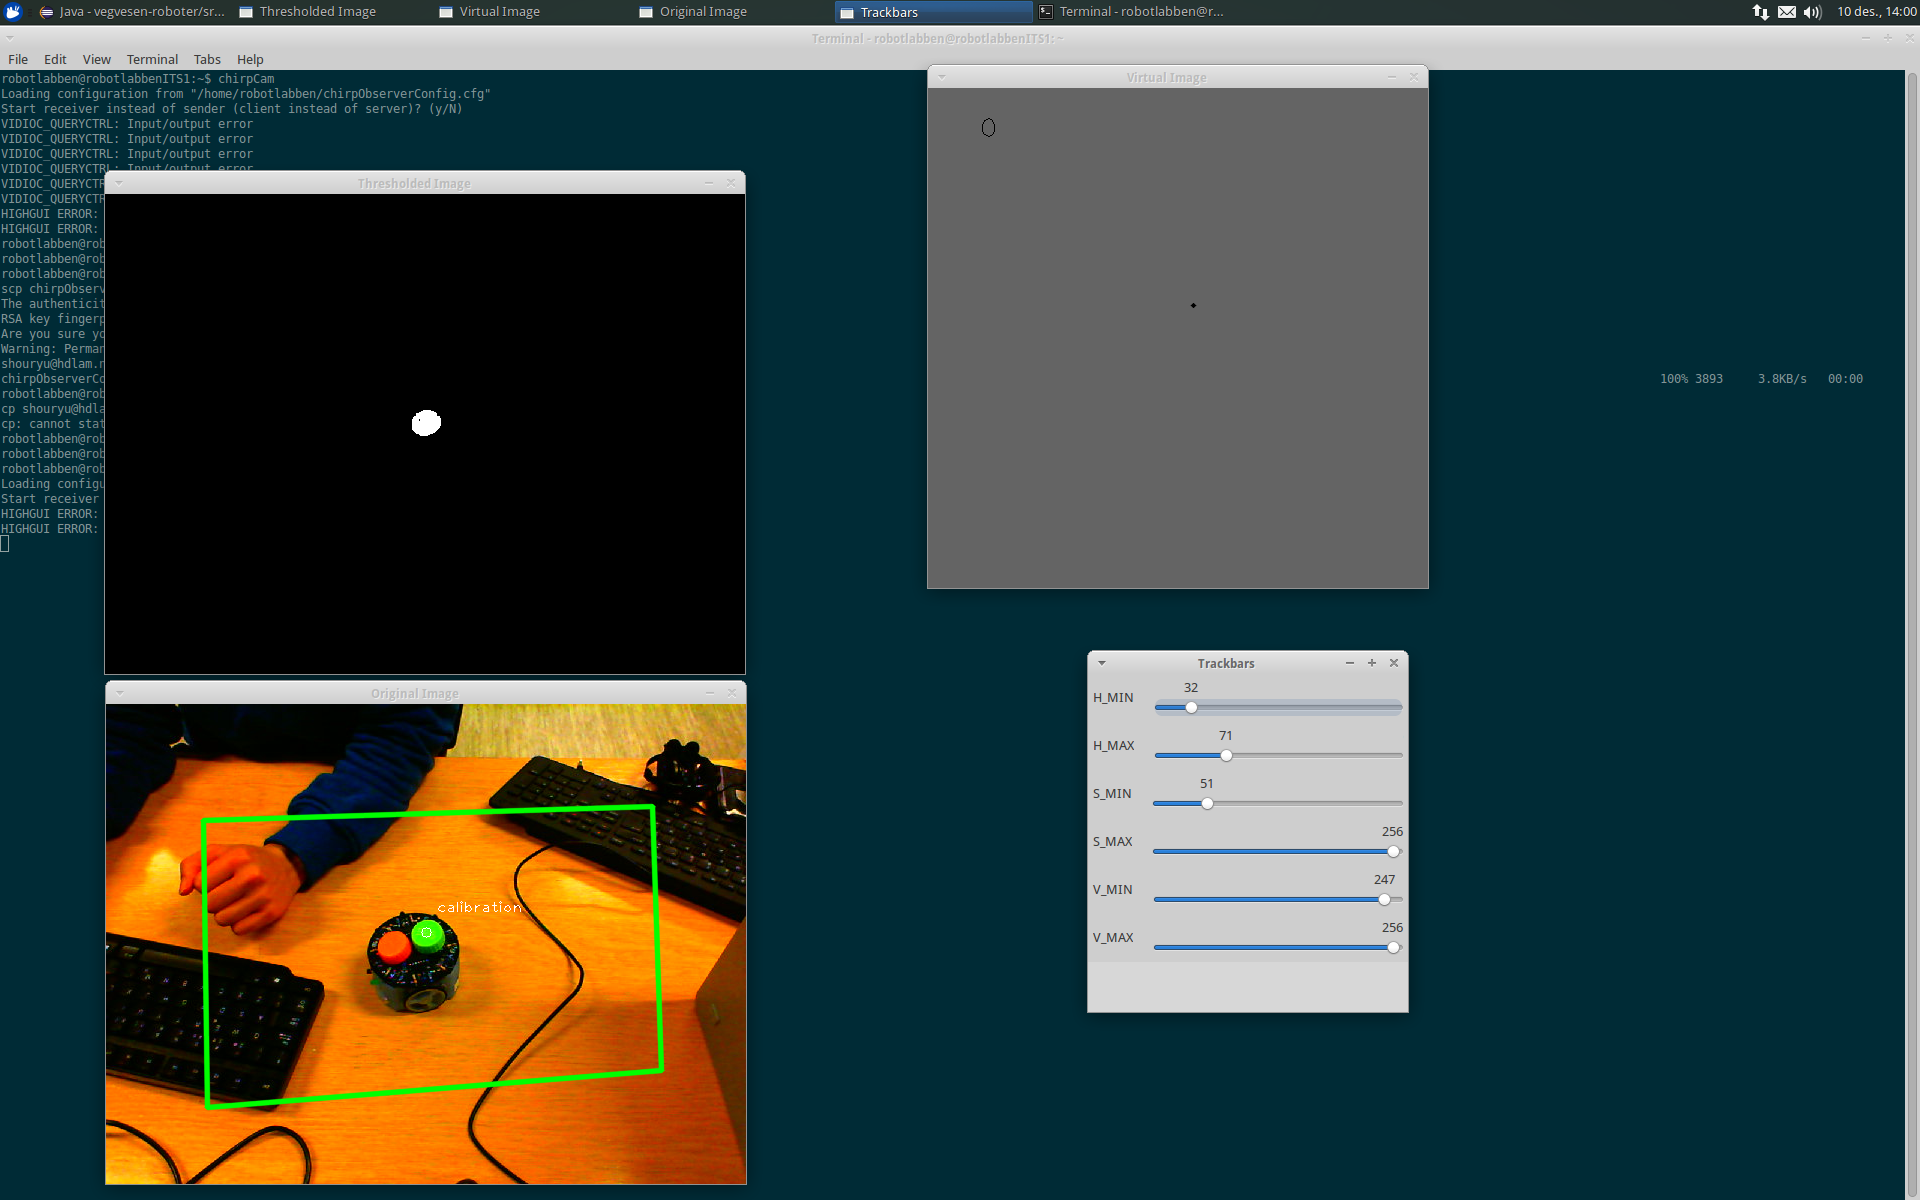
\includegraphics[width=0.8\linewidth]{images/calibration.png}
\caption[calibration of the camera tracking software]{The upper left window shows us which dots are considered the current color, HSV, Chirp, window}
\end{figure}

The position and rotation of each robot was then sent to the simulation written in Java via UDP packets as a string, which the simulation decomposed using regular expression and converted to meaningful data which could be set for each robot. Due to the high update frequency of the camera, the simulator had to average each 5 position and rotation it got from the camera software. This was done to avoid jiggling due to noise. We had some problems with the camera software not working without an internet connection, the program would crash if the computer did not have an internet connection with the error message "seg fault". The program needed it to send the packets over UDP, we had both camera software and Java simulation on the same machine, so the UDP packets were only sent to itself (localhost) so we did not really need a internet connection, but the software believed that it needed one. We fixed this problem by connecting a ethernet cable between the host machine and the computer nearby, that would trick the program thinking that it had a valid connection.

Another problem that was present was the ID of the robot, each robot would have an unique ID. When one of the robot went out of sight - that is the camera is being covered or the robot drove outside of its range, the camera software would assign new ID to all of the robots. For instance if we have 2 robots with the ID 0 and ID 1. If robot1 cannot be tracked by the camera then robot0 will get ID 2 and counting until the original robot1 reenters the frame. So at one point the robots might have the ID 7 and 8. The Java simulation uses these ID to keep track of the robots, and which COM port belongs to which ID. The simulator did still know approximately where each robot were supposed to be before the camera lost track of it, so when a robot would disappear and reappear with a new ID, the simulator would simply find the nearest robot and reassign the new ID to that robot.

The simulation then calculated where the robot needed to go, set the speed for each wheel and sent the commands to the robot using the bluetooth COM-port.

The Java simulation was first implemented by Magnus Hu using a game framework called Lightweight Java Game Library (LWJGL) to render everything on screen. We decided to change the framework from LWJGL to Slick2D. Slick2D is a 2D Java game library which uses tools and utilities wrapped around LWJGL, which means that it can do everything LWJGL can do, but also has higher abstraction. Slick2D lets us render shapes (circles, squares) without having to specify each point and line of the shape manually which we had to do in LWJGL. We could also easily check if the shapes intersected each other using the built in method "intersects" for the Shape class. In LWJGL, the robots were rendered as triangle by using 4 points, where 2 of the points would overlap. This was hard to build upon and it did not give an accurate model of how the robot looks in real life .
In Slick2D we rendered a circle shape for each robot with a square cone in front of it and a bit larger circle shape around the robot. The square cone was used as the vision of the robot, and the outer circular shape was used to detect when robots were too close to each other. If these out circles intersected the robot were forced to stop immediately because they are likely to crash into each other.\\


The track used in the simulation consisted of 24 points (a point as in a point in space) laid out in a 8-shaped layout, where the center intersection is made up of 2 points. For every point in the list, a line would be drawn between a point and its 2 neighbors in the list, this formed the 8-shaped figure which was our track.
A prototype image of a 8 shaped track that we got from Vegvesenet was used to find the 24 points. 
Our demo at Teknologidagene used 4 robots because we only had 4 bluetooth modules. The bluetooth modules had to be connected and added manually as a COM port before running the simulation or else it wouldn't know where to send the commands. When starting both the OpenCV camera tracking software and the simulation, the ID, coordinates of each robot and the rotation/alignment were tracked and sent via UDP packets. At this point in time, the simulation doesn't know which coordinate and rotation belongs to which bluetooth COM port. To map the COM port to a robot the simulator does the following for each robot:
\begin{itemize}
    \item checks the angle of all the robots
    \item sends a rotate command to the bluetooth COM port, which makes one robot rotate approximately 90 degrees.
    \item checks the angle of all the robots, finds out which one has rotated the most, saves this COM port to the robot which have rotated the most
    \item rotates the robot back to the original orientation
\end{itemize}
The reason for rotating the robot back to the original orientation is because we always laid the robot out in the map facing forward, which was easier to implement instead of implementing a lot of code to ensure that the robot would face forward if it started out in the wrong direction.
Each robot will now have a COM port given that the COM port didn't time out on initiation, in which we had to restart the whole simulation program to reconnect to the COM port.
The simulation then calculates the robot's nearest point on the track, and sets the target point of the robot to be point after the nearest one, this is in case the nearest point is behind the robot. After the simulation found out where the robot should move to, it calculates which way the robot needed to rotate and which speed it should have. The speed and the amount of needed rotation ($\Delta angle$) is then converted to <"two motors"> which is sent as a byte array of 4 elements to the robot's bluetooth module. An example of the byte array could be "l40r50" which means that the right motor would drive a little bit faster than the left one thus turning the robot to the left.
If we used a capital 'L' or 'R' in the byte array instead, the wheel would turn backwards, however we don't use that in the simulation at all except for turning the robot in the beginning when it tries to assign the COM port to the correct robot.

The simulator creates a box in front of each robot that will be used to find out whether the robot has a robot in front of it or not. If there is a robot in front (that is inside the front box) then the simulator will check if platooning is on or not. If platooning mode is on, the robot will try to keep the same speed as the robot in front of it. At least it's not allowed to have higher speed than the robot in front of it, or else it will crash into it. If platooning mode is off, then the robot will try to keep a 3 second distance from the robot in front, that is the robot will try to keep the robot in front of it outside the detection box. The robot is considered as reaching a target if the robot's center is 20 pixels away from the target, and the next point will be assigned as the new target for the robot.
The simulator have two modes for the robot, one where platooning is activated and one mode where the robots behave like normal cars. The normal car mode is emulating how drivers would drive normally. In front of each robot in the simulation there would be rendered a square cone-shaped shape which would be larger when the robot had high speed and smaller if the robot had slower speed. The shape would be almost non existing if the robot were to stand completely still. This shape would tell the robot that there is another robot in front of it, and the current robot would try to adjust it speed so the robot in front is outside of this "detector" shape. This shape is supposed to be a three second rule, and would let the robot brake without having to brake heavily.
In platooning mode on the other hand, the robots will extend their shape a lot further than it did in normal drive mode. This shape will now be used to ask the robots inside of it what speed they have, and if they're braking or not.
If the robot in front have a max speed $x$ then the robot behind can only drive as fast as $x$, a higher speed would make the robot crash or bump into each other.
The robot in the back will always ask the robot in front if it is braking or not, if the robot in front says that it is currently braking, then the robot behind would also brake immediately.
In our implementation we had to cheat the platooning algorithm a bit, due to the delays in the bluetooth signals and how fast the robots are able to react. If we sent a new command too rapidly, the robot would not move because a new command would overwrite the old command before the motors were able to issue the old command. So we had to insert a delay between sending each command to the robots, we were only allowed to send a command 5 times each second. This was enough to make the platooned robots fall a little bit behind the robot in front of it, so it did not seem like they platooned at all. The fix we implemented was to have the cars behind try to catch up to the robot in front of it if the current mode was platooning mode. This fix made the robots look more like they actually were platooning.\\

Some other problems we had under the demonstration was some of the styrofoam buildings used around the tracks were too tall, and covered the robots when they rounded the turn. When we cut down the tallest building, it was still casting shadows on to the track. The shadow made the robot's post it note have a different shade of green/pink, and the camera lost track of it. We had to cut the building even more so the shadow didn't reach the track.


In the middle of the map, at the intersection there is a red light at the top, north side or at the right, east side of the intersection. This red light will be alternating between these two positions depending on what the user chooses. 

Most of the codes written for this platooning demo was already implemented or had already been started on, the code for the robot tracking written in C++ with the openCV and boost library. The libraries for the ChIRP robot already existed, Christian Skjetne implemented the code using Arduino language on the robot which used the bluetooth module. 
I did not get to code so much on the robots itself, but next semester I will be a student assistant in the new course for the first grader in computer science named programming lab where they are supposed to program on the Arduino. So this year I have been attending two courses that focused on learning input sensors and getting to know the Arduino. One of the main thing in that course is the bluetooth low energy module, which is pretty similar to the bluetooth used on the ChIRPs. 
